\usepackage[dvipsnames]{xcolor}
\usepackage[utf8]{inputenc}
\usepackage[T1]{fontenc}
\usepackage{geometry}
\geometry{
    top=1cm,
    bottom=1.5cm,
    left=4.5cm,
    right=4.5cm,
    includehead,
    includefoot,
}
\usepackage{lastpage}
\usepackage[font={small,sf},labelfont={bf}]{caption}
\usepackage{nameref}
\usepackage{makecell}
\usepackage[all]{nowidow}
\usepackage[hidelinks]{hyperref}

\usepackage{bm}


\newcommand{\xset}{\mathbb{X}}
\newcommand{\xseti}{\mathbb{X}^{(i)}}
\newcommand{\approxdistri}{q_{\phi}(\textbf{z}|\xseti)}
\newcommand{\approxdistr}{q_{\phi}(\textbf{z}|\xset)}
\newcommand{\truedistr}{p_{\theta}(\textbf{z}|\xseti)}
\newcommand{\elbo}{\mathcal{L}(\theta, \phi; \xseti)}
\newcommand{\xsubset}{\mathbb{X}_k}
\newcommand{\lmopoe}{\mathcal{L}_{MoPoE}(\theta, \phi; \xset)}
\newcommand{\powerset}{\mathcal{P}(\xset)}

\usepackage{graphicx}
\usepackage{hyperref}
\usepackage{cleveref}

\usepackage{amsfonts}
\usepackage{abstract} % Allows abstract customization
\renewcommand{\abstractnamefont}{\normalfont\bfseries} % Set the "Abstract" text to bold
\renewcommand{\abstracttextfont}{\normalfont\small\itshape} % Set the abstract itself to small italic text

%experiments variables
\newcommand{\imgsize}{(128, 128)}
\newcommand{\minwordocc}{3 }
\newcommand{\sentlen}{128 }
\newcommand{\learningrate}{0.001}

% Article-specific configuration
\begin{pythontexcustomcode}[begin]{py}
    DOC_STYLE="article/main.conf"
    pytex.add_dependencies(DOC_STYLE)
\end{pythontexcustomcode}

%VARIABLES
%set up a more stable buffers (the normal ones gets blanked after the titlepage is invoked)
\makeatletter
\let\mytitle\@title
\let\myauthor\@author
\let\mydate\@date
\makeatother


%TITLE
\usepackage{authblk}
\renewcommand\Affilfont{\itshape\small}

\newcommand{\authorstyle}[1]{{\large\bfseries\textsf{\color{Gray}#1}}}


% Sections
% make sure the first paragraph of a section is not indented
\makeatletter
\let\@afterindenttrue\@afterindentfalse
\@afterindentfalse
\makeatother

%\usepackage[explicit]{titlesec}
%\titleformat{\section}[hang]{\Large\usefont{T1}{phv}{b}{n}\color{Black}}{}{0em}{#1}%
%\titlespacing{\section}{0em}{1.5em}{0.4em}
%\titleformat{\subsection}[hang]{\usefont{T1}{phv}{b}{n}\color{Black}}{}{0em}{#1}%
%\titlespacing{\subsection}{0em}{1em}{0.2em}
%\titleformat{\subsubsection}[hang]{\footnotesize\usefont{T1}{phv}{b}{n}\color{Black}}{}{0em}{#1}%
%\titlespacing{\subsubsection}{0em}{0.75em}{0em}


% Grey definitions.
\definecolor{dg}{gray}{0.25}
\definecolor{mg}{gray}{0.55}
\definecolor{lg}{gray}{0.73}
\definecolor{vlg}{gray}{0.9}

% Boilerplate visual style improvements
\newcommand{\niceus}{\texttt{\_}}




\title{Multimodal Generative Learning on the MIMIC-CXR Database}
\subtitle{A presentation of my semester project}
\author{Hendrik Klug}
\institute{Institute for Electrical Engineering, ETH}
\begin{document}
	\begin{frame}
		\titlepage
	\end{frame}
	\section{Introduction}

	    \begin{frame}
	        In this work, we applied a method for self-supervised, multimodal and generative training from \cite{thomas_multimodal} on the MIMIC-CXR Database \cite{johnson2019mimic}.
	    \end{frame}

		\subsection{Multimodal, Unsupervised, Generative models}
			\begin{frame}{The General Idea}
				\py{pytex_printonly(script='scripts/generalidea_graph.py', data = '')}
			\end{frame}

        \begin{frame}{Multimodal, Unsupervised Generative Learning On Medical Data}
            \begin{itemize}
                \item No need for labeled data
                \item Can extract features from multiple modalities
                \item Can generate \textit{coherent} samples from one input modality
            \end{itemize}
        \end{frame}

    \section{Background}
        \subsection{The MoPoE-VAE}
            \begin{frame}{The Mixture-of-Products-of-Experts-VAE}
            Combination of:
                \begin{itemize}
                    \item The Product-of-Experts (PoE) from \cite{wu2018multimodal}
                    \item The Mixture-of-Experts (MoE) from \cite{shi2019variational}
                \end{itemize}
                \vspace{\baselineskip}
                Both differ in their choice of the joint posterior approximation functions.
            \end{frame}

            \begin{frame}{The PoE-VAE}

                \begin{itemize}
                    \item Uses a geometric mean: the joint posterior is a product of individual posteriors
                    %p(z|x_1,...,x_N)) \propto p(z) \prod _{i=1} ^N \tilde{q}(z|x_i)
                \begin{equation}
                    q_{\Phi}(z|x_{1:M})=\prod _m q_{\Phi_m}(z|x_m)
                \end{equation}
                    \item Results in a good approximation of the joint distribution but struggles in optimizing the individual experts.
                \end{itemize}

            \end{frame}

            \begin{frame}{The MoE-VAE}
            \begin{itemize}
                \item Uses an arithmetic mean
                \begin{equation}
                    q_{\Phi}(z|x_{1:M})=\sum _m \alpha_m\cdot q_{\Phi_m}(z|x_m)
                \end{equation}
                \item Optimizes individual experts well but is not able to learn a distribution that is sharper than any of its experts.
            \end{itemize}

            \end{frame}

            \begin{frame}{The Mixture-of-Products-of-Experts-VAE}
                The generalized multimodal ELBO utilizes the PoE to get the posterior approximation of a subset $\xsubset \in \mathcal{P}(\mathbb{X})$:

				\begin{equation}
					\tilde{q}_{\phi}(\textbf{z}|\xsubset)=PoE(\{q_{\phi_j}(\textbf{z}|\textbf{x}_j) \forall \textbf{x}_j \in \xsubset\}) \propto \prod _{\textbf{x}_j \in \xsubset}q_{\phi_j}(\textbf{z}|\textbf{x}_j)
				\end{equation}
				And the MoE to get the joint posterior:
				\begin{equation}
					q_{\phi}(\textbf{z}|\mathbb{X}) = \frac{1}{2^3} \sum _{\textbf{x}_k \in \mathbb{X}} \tilde{q}_{\phi} (\textbf{z}|\mathbb{X}_k)
				\end{equation}
            \end{frame}

            \begin{frame}{Frame Title}

			\py{pytex_printonly(script='scripts/mopoe_graph.py', data = '')}

            \end{frame}

    \section{Methods}
        \subsubsection{The MIMIC-CXR Database}
            \begin{frame}{The dataset}
            The MIMIC-CXR Database \cite{johnson2019mimic} is a large publicly available dataset of chest radiographs with free-text radiology reports containing 377,110 images corresponding to 227,835 radiographic studies performed at the Beth Israel Deaconess Medical Center in Boston, MA.
                
            \end{frame}
            
            \begin{frame}
                \begin{enumerate}
                    \item Implemented word encoding (show dictionary example)
                    \item tested image size
                    \item tested beta
                    \item tested class dim
                \end{enumerate}
            \end{frame}

            \begin{frame}
                \py{pytex_fig('scripts/rand_sample_from_dataset.py', conf='slides/dataset.conf', label='dataset_samples', caption='Samples from the dataset.')}
            \end{frame}
            
            \begin{frame}{The labels}
                Since the multiple labels from the dataset are highly imbalanced, we created a label "Finding", indicating if the sample is labeled with any pathology.\\
                There are \py{boilerplate.print_finding_counts()} samples that are annotated with the "Finding" label in the training set and \py{boilerplate.print_nofinding_counts()} samples that are not.
            \end{frame}
            
            \begin{frame}{The word encoding}
                Every word that occurs at least \py{boilerplate.print_flag_attribute('word_min_occ')} times in all the text reports is mapped to an index.\\
                Using this mapping each sentence is encoded into a sequence of indices.\\
                
                \pause
                "Heart size is normal." $\rightarrow [0,1,2,3] \rightarrow$ Model $\rightarrow
                \begin{bmatrix}
                1 & 0 & 0 & 0\\
                0 & 1 & 0 & 0\\
                0 & 0 & 1 & 0\\
                0 & 0 & 0 & 1\\
                \end{bmatrix}$\\
                $\rightarrow [0,1,2,3] \rightarrow$ "Heart size is normal." 
            \end{frame}
            
        \subsection{The model architecture}
        \begin{frame}{The model}
            The MoPoE-VAE has an encoder and decoder for each modality, in this work both are the same for the image modalities (frontal and lateral scans).
        \end{frame}
        
        \begin{frame}{Resnet}
        % todo
        Show resnet architecture
            
        \end{frame}
        
        \subsection{Evaluation methods}
        \begin{frame}{Evaluation of the latent representation}
        \begin{figure}[!h]
        \centering
        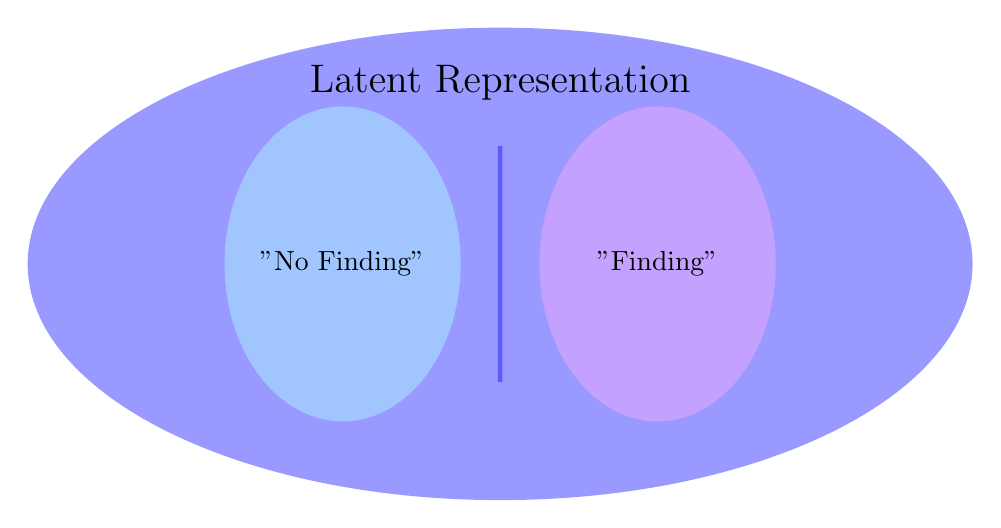
\begin{tikzpicture}
        
              \begin{scope}[blend group = soft light]
                \fill[blue!40!white]   (0:0) ellipse (6cm and 3cm);
                \fill[green!40!white] (0:-2) ellipse (1.5cm and 2cm);
                \fill[red!40!white]  (0:2) ellipse (1.5cm and 2cm);
                \draw [-,ultra thick] (0,-1.5) -- (0,1.5);
            \end{scope}
                \node at (0:-2)   {"No Finding"};
              \node at (0:2)   {"Finding"};
              \node at (90:2.3) [font=\Large] {Latent Representation};
            \end{tikzpicture}
        \end{figure}    
        \end{frame}
        
        \begin{frame}{Evaluation of the generation coherence}
        To evaluate the coherence of the generated samples, they are classified using trained ResNet classifiers.
        If all modalities of a sample, generated and given as conditioner, are classified as having the same label, they are considered coherent.
        \end{frame}
        
    \section{Results}
        \subsection{Generation Evaluation}
        
    
        
\printbibliography
\end{document}
